\begin{figure}[H]
	\centering
	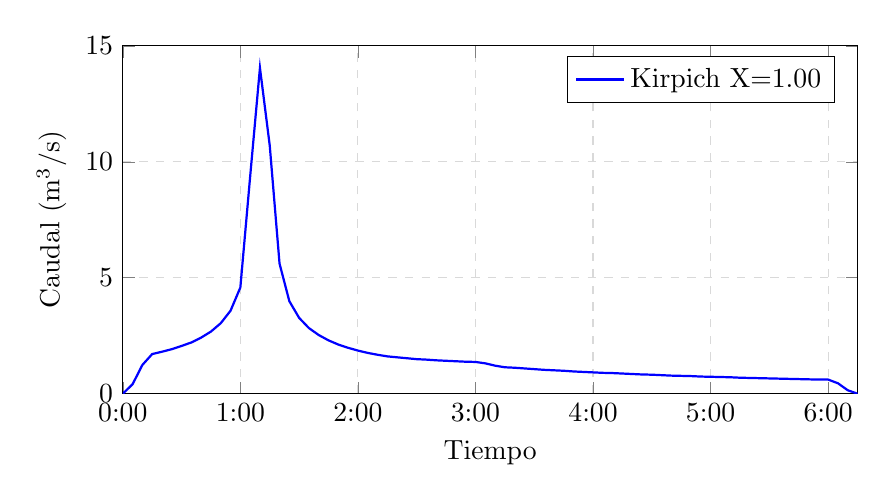
\begin{tikzpicture}
		\begin{axis}[
			width=0.9\textwidth,
			height=6cm,
			xlabel={Tiempo},
			ylabel={Caudal (m$^3$/s)},
			xmin=0,
			xmax=375,
			ymin=0,
			ymax=15,
			grid=major,
			grid style={dashed, gray!30},
			legend pos=north east,
			xtick={0, 60, 120, 180, 240, 300, 360},
			xticklabels={0:00, 1:00, 2:00, 3:00, 4:00, 5:00, 6:00},
			]
		% Kirpich X=1.00
		\addplot [
		blue,
		thick,
		solid,
		] coordinates {
				(0, 0.00) (5, 0.41) (10, 1.24) (15, 1.71) (20, 1.81)
				(25, 1.92) (30, 2.06) (35, 2.21) (40, 2.42) (45, 2.68)
				(50, 3.04) (55, 3.58) (60, 4.58) (65, 9.36) (70, 14.05)
				(75, 10.70) (80, 5.61) (85, 3.99) (90, 3.27) (95, 2.83)
				(100, 2.53) (105, 2.30) (110, 2.12) (115, 1.98) (120, 1.86)
				(125, 1.76) (130, 1.68) (135, 1.61) (140, 1.57) (145, 1.53)
				(150, 1.49) (155, 1.47) (160, 1.44) (165, 1.42) (170, 1.40)
				(175, 1.38) (180, 1.37) (185, 1.31) (190, 1.21) (195, 1.14)
				(200, 1.12) (205, 1.09) (210, 1.06) (215, 1.03) (220, 1.01)
				(225, 0.99) (230, 0.96) (235, 0.94) (240, 0.92) (245, 0.90)
				(250, 0.89) (255, 0.87) (260, 0.85) (265, 0.83) (270, 0.82)
				(275, 0.80) (280, 0.78) (285, 0.77) (290, 0.76) (295, 0.74)
				(300, 0.73) (305, 0.72) (310, 0.71) (315, 0.69) (320, 0.68)
				(325, 0.67) (330, 0.66) (335, 0.65) (340, 0.64) (345, 0.63)
				(350, 0.62) (355, 0.61) (360, 0.61) (365, 0.45) (370, 0.15)
				(375, 0.00)
		};
		\addlegendentry{Kirpich X=1.00}

		\end{axis}
	\end{tikzpicture}
	\caption{Hidrograma - Kirpich + GZ $T_r$=10 años ($Q_p$=14.047 m$^3$/s)}
	\label{fig:hydro_kirpich_gz_Tr10_X100}
\end{figure}
